\documentclass{article}

\usepackage{graphicx}
\usepackage{amsmath}
\usepackage{fancyhdr}
\usepackage{hyperref}
\usepackage[dvipsnames]{xcolor}
\usepackage{enumitem}
\usepackage{minted}
%%%%% NEW MATH DEFINITIONS %%%%%

\usepackage{amsmath,amsfonts,bm,bbm}

\def\ind{{\mathbbm{1}}}

% Mark sections of captions for referring to divisions of figures
\newcommand{\figleft}{{\em (Left)}}
\newcommand{\figcenter}{{\em (Center)}}
\newcommand{\figright}{{\em (Right)}}
\newcommand{\figtop}{{\em (Top)}}
\newcommand{\figbottom}{{\em (Bottom)}}
\newcommand{\captiona}{{\em (a)}}
\newcommand{\captionb}{{\em (b)}}
\newcommand{\captionc}{{\em (c)}}
\newcommand{\captiond}{{\em (d)}}
\newcommand{\figleftt}{{\em Left}}
\newcommand{\figcentert}{{\em Center}}
\newcommand{\figrightt}{{\em Right}}
\newcommand{\figtopt}{{\em Top}}
\newcommand{\figbottomt}{{\em Bottom}}
\newcommand{\captionat}{{\em a}}
\newcommand{\captionbt}{{\em b}}
\newcommand{\captionct}{{\em c}}
\newcommand{\captiondt}{{\em d}}

% Highlight a newly defined term
\newcommand{\newterm}[1]{{\bf #1}}


% Figure reference, lower-case.
\def\figref#1{figure~\ref{#1}}
% Figure reference, capital. For start of sentence
\def\Figref#1{Figure~\ref{#1}}
\def\twofigref#1#2{figures \ref{#1} and \ref{#2}}
\def\quadfigref#1#2#3#4{figures \ref{#1}, \ref{#2}, \ref{#3} and \ref{#4}}
% Section reference, lower-case.
\def\secref#1{section~\ref{#1}}
% Section reference, capital.
\def\Secref#1{Section~\ref{#1}}
% Reference to two sections.
\def\twosecrefs#1#2{sections \ref{#1} and \ref{#2}}
% Reference to three sections.
\def\secrefs#1#2#3{sections \ref{#1}, \ref{#2} and \ref{#3}}

\def\chapref#1{chapter~\ref{#1}}
% Reference to an equation, upper case.
\def\Chapref#1{Chapter~\ref{#1}}
% Reference to a range of chapters
\def\rangechapref#1#2{chapters\ref{#1}--\ref{#2}}
% Reference to an algorithm, lower-case.
\def\algref#1{algorithm~\ref{#1}}
% Reference to an algorithm, upper case.
\def\Algref#1{Algorithm~\ref{#1}}
\def\twoalgref#1#2{algorithms \ref{#1} and \ref{#2}}
\def\Twoalgref#1#2{Algorithms \ref{#1} and \ref{#2}}
% Reference to a part, lower case
\def\partref#1{part~\ref{#1}}
% Reference to a part, upper case
\def\Partref#1{Part~\ref{#1}}
\def\twopartref#1#2{parts \ref{#1} and \ref{#2}}

\def\ceil#1{\lceil #1 \rceil}
\def\floor#1{\lfloor #1 \rfloor}
\def\1{\bm{1}}
\newcommand{\train}{\mathcal{D}}
\newcommand{\valid}{\mathcal{D_{\mathrm{valid}}}}
\newcommand{\test}{\mathcal{D_{\mathrm{test}}}}

\def\eps{{\epsilon}}


% Random variables
\def\reta{{\textnormal{$\eta$}}}
\def\ra{{\textnormal{a}}}
\def\rb{{\textnormal{b}}}
\def\rc{{\textnormal{c}}}
\def\rd{{\textnormal{d}}}
\def\re{{\textnormal{e}}}
\def\rf{{\textnormal{f}}}
\def\rg{{\textnormal{g}}}
\def\rh{{\textnormal{h}}}
\def\ri{{\textnormal{i}}}
\def\rj{{\textnormal{j}}}
\def\rk{{\textnormal{k}}}
\def\rl{{\textnormal{l}}}
% rm is already a command, just don't name any random variables m
\def\rn{{\textnormal{n}}}
\def\ro{{\textnormal{o}}}
\def\rp{{\textnormal{p}}}
\def\rq{{\textnormal{q}}}
\def\rr{{\textnormal{r}}}
\def\rs{{\textnormal{s}}}
\def\rt{{\textnormal{t}}}
\def\ru{{\textnormal{u}}}
\def\rv{{\textnormal{v}}}
\def\rw{{\textnormal{w}}}
\def\rx{{\textnormal{x}}}
\def\ry{{\textnormal{y}}}
\def\rz{{\textnormal{z}}}

% Random vectors
\def\rvepsilon{{\mathbf{\epsilon}}}
\def\rvtheta{{\mathbf{\theta}}}
\def\rva{{\mathbf{a}}}
\def\rvb{{\mathbf{b}}}
\def\rvc{{\mathbf{c}}}
\def\rvd{{\mathbf{d}}}
\def\rve{{\mathbf{e}}}
\def\rvf{{\mathbf{f}}}
\def\rvg{{\mathbf{g}}}
\def\rvh{{\mathbf{h}}}
\def\rvu{{\mathbf{i}}}
\def\rvj{{\mathbf{j}}}
\def\rvk{{\mathbf{k}}}
\def\rvl{{\mathbf{l}}}
\def\rvm{{\mathbf{m}}}
\def\rvn{{\mathbf{n}}}
\def\rvo{{\mathbf{o}}}
\def\rvp{{\mathbf{p}}}
\def\rvq{{\mathbf{q}}}
\def\rvr{{\mathbf{r}}}
\def\rvs{{\mathbf{s}}}
\def\rvt{{\mathbf{t}}}
\def\rvu{{\mathbf{u}}}
\def\rvv{{\mathbf{v}}}
\def\rvw{{\mathbf{w}}}
\def\rvx{{\mathbf{x}}}
\def\rvy{{\mathbf{y}}}
\def\rvz{{\mathbf{z}}}

% Elements of random vectors
\def\erva{{\textnormal{a}}}
\def\ervb{{\textnormal{b}}}
\def\ervc{{\textnormal{c}}}
\def\ervd{{\textnormal{d}}}
\def\erve{{\textnormal{e}}}
\def\ervf{{\textnormal{f}}}
\def\ervg{{\textnormal{g}}}
\def\ervh{{\textnormal{h}}}
\def\ervi{{\textnormal{i}}}
\def\ervj{{\textnormal{j}}}
\def\ervk{{\textnormal{k}}}
\def\ervl{{\textnormal{l}}}
\def\ervm{{\textnormal{m}}}
\def\ervn{{\textnormal{n}}}
\def\ervo{{\textnormal{o}}}
\def\ervp{{\textnormal{p}}}
\def\ervq{{\textnormal{q}}}
\def\ervr{{\textnormal{r}}}
\def\ervs{{\textnormal{s}}}
\def\ervt{{\textnormal{t}}}
\def\ervu{{\textnormal{u}}}
\def\ervv{{\textnormal{v}}}
\def\ervw{{\textnormal{w}}}
\def\ervx{{\textnormal{x}}}
\def\ervy{{\textnormal{y}}}
\def\ervz{{\textnormal{z}}}

% Random matrices
\def\rmA{{\mathbf{A}}}
\def\rmB{{\mathbf{B}}}
\def\rmC{{\mathbf{C}}}
\def\rmD{{\mathbf{D}}}
\def\rmE{{\mathbf{E}}}
\def\rmF{{\mathbf{F}}}
\def\rmG{{\mathbf{G}}}
\def\rmH{{\mathbf{H}}}
\def\rmI{{\mathbf{I}}}
\def\rmJ{{\mathbf{J}}}
\def\rmK{{\mathbf{K}}}
\def\rmL{{\mathbf{L}}}
\def\rmM{{\mathbf{M}}}
\def\rmN{{\mathbf{N}}}
\def\rmO{{\mathbf{O}}}
\def\rmP{{\mathbf{P}}}
\def\rmQ{{\mathbf{Q}}}
\def\rmR{{\mathbf{R}}}
\def\rmS{{\mathbf{S}}}
\def\rmT{{\mathbf{T}}}
\def\rmU{{\mathbf{U}}}
\def\rmV{{\mathbf{V}}}
\def\rmW{{\mathbf{W}}}
\def\rmX{{\mathbf{X}}}
\def\rmY{{\mathbf{Y}}}
\def\rmZ{{\mathbf{Z}}}
\def\rmtheta{{\mathbf{\Theta}}}
% Elements of random matrices
\def\ermA{{\textnormal{A}}}
\def\ermB{{\textnormal{B}}}
\def\ermC{{\textnormal{C}}}
\def\ermD{{\textnormal{D}}}
\def\ermE{{\textnormal{E}}}
\def\ermF{{\textnormal{F}}}
\def\ermG{{\textnormal{G}}}
\def\ermH{{\textnormal{H}}}
\def\ermI{{\textnormal{I}}}
\def\ermJ{{\textnormal{J}}}
\def\ermK{{\textnormal{K}}}
\def\ermL{{\textnormal{L}}}
\def\ermM{{\textnormal{M}}}
\def\ermN{{\textnormal{N}}}
\def\ermO{{\textnormal{O}}}
\def\ermP{{\textnormal{P}}}
\def\ermQ{{\textnormal{Q}}}
\def\ermR{{\textnormal{R}}}
\def\ermS{{\textnormal{S}}}
\def\ermT{{\textnormal{T}}}
\def\ermU{{\textnormal{U}}}
\def\ermV{{\textnormal{V}}}
\def\ermW{{\textnormal{W}}}
\def\ermX{{\textnormal{X}}}
\def\ermY{{\textnormal{Y}}}
\def\ermZ{{\textnormal{Z}}}

% Vectors
\def\vzero{{\bm{0}}}
\def\vone{{\bm{1}}}
\def\vmu{{\bm{\mu}}}
\def\vtheta{{\bm{\theta}}}
\def\va{{\bm{a}}}
\def\vb{{\bm{b}}}
\def\vc{{\bm{c}}}
\def\vd{{\bm{d}}}
\def\ve{{\bm{e}}}
\def\vf{{\bm{f}}}
\def\vg{{\bm{g}}}
\def\vh{{\bm{h}}}
\def\vi{{\bm{i}}}
\def\vj{{\bm{j}}}
\def\vk{{\bm{k}}}
\def\vl{{\bm{l}}}
\def\vm{{\bm{m}}}
\def\vn{{\bm{n}}}
\def\vo{{\bm{o}}}
\def\vp{{\bm{p}}}
\def\vq{{\bm{q}}}
\def\vr{{\bm{r}}}
\def\vs{{\bm{s}}}
\def\vt{{\bm{t}}}
\def\vu{{\bm{u}}}
\def\vv{{\bm{v}}}
\def\vw{{\bm{w}}}
\def\vx{{\bm{x}}}
\def\vy{{\bm{y}}}
\def\vz{{\bm{z}}}

% Elements of vectors
\def\evalpha{{\alpha}}
\def\evbeta{{\beta}}
\def\evepsilon{{\epsilon}}
\def\evlambda{{\lambda}}
\def\evomega{{\omega}}
\def\evmu{{\mu}}
\def\evpsi{{\psi}}
\def\evsigma{{\sigma}}
\def\evtheta{{\theta}}
\def\eva{{a}}
\def\evb{{b}}
\def\evc{{c}}
\def\evd{{d}}
\def\eve{{e}}
\def\evf{{f}}
\def\evg{{g}}
\def\evh{{h}}
\def\evi{{i}}
\def\evj{{j}}
\def\evk{{k}}
\def\evl{{l}}
\def\evm{{m}}
\def\evn{{n}}
\def\evo{{o}}
\def\evp{{p}}
\def\evq{{q}}
\def\evr{{r}}
\def\evs{{s}}
\def\evt{{t}}
\def\evu{{u}}
\def\evv{{v}}
\def\evw{{w}}
\def\evx{{x}}
\def\evy{{y}}
\def\evz{{z}}

% Matrix
\def\mA{{\bm{A}}}
\def\mB{{\bm{B}}}
\def\mC{{\bm{C}}}
\def\mD{{\bm{D}}}
\def\mE{{\bm{E}}}
\def\mF{{\bm{F}}}
\def\mG{{\bm{G}}}
\def\mH{{\bm{H}}}
\def\mI{{\bm{I}}}
\def\mJ{{\bm{J}}}
\def\mK{{\bm{K}}}
\def\mL{{\bm{L}}}
\def\mM{{\bm{M}}}
\def\mN{{\bm{N}}}
\def\mO{{\bm{O}}}
\def\mP{{\bm{P}}}
\def\mQ{{\bm{Q}}}
\def\mR{{\bm{R}}}
\def\mS{{\bm{S}}}
\def\mT{{\bm{T}}}
\def\mU{{\bm{U}}}
\def\mV{{\bm{V}}}
\def\mW{{\bm{W}}}
\def\mX{{\bm{X}}}
\def\mY{{\bm{Y}}}
\def\mZ{{\bm{Z}}}
\def\mBeta{{\bm{\beta}}}
\def\mPhi{{\bm{\Phi}}}
\def\mLambda{{\bm{\Lambda}}}
\def\mSigma{{\bm{\Sigma}}}

% Tensor
\DeclareMathAlphabet{\mathsfit}{\encodingdefault}{\sfdefault}{m}{sl}
\SetMathAlphabet{\mathsfit}{bold}{\encodingdefault}{\sfdefault}{bx}{n}
\newcommand{\tens}[1]{\bm{\mathsfit{#1}}}
\def\tA{{\tens{A}}}
\def\tB{{\tens{B}}}
\def\tC{{\tens{C}}}
\def\tD{{\tens{D}}}
\def\tE{{\tens{E}}}
\def\tF{{\tens{F}}}
\def\tG{{\tens{G}}}
\def\tH{{\tens{H}}}
\def\tI{{\tens{I}}}
\def\tJ{{\tens{J}}}
\def\tK{{\tens{K}}}
\def\tL{{\tens{L}}}
\def\tM{{\tens{M}}}
\def\tN{{\tens{N}}}
\def\tO{{\tens{O}}}
\def\tP{{\tens{P}}}
\def\tQ{{\tens{Q}}}
\def\tR{{\tens{R}}}
\def\tS{{\tens{S}}}
\def\tT{{\tens{T}}}
\def\tU{{\tens{U}}}
\def\tV{{\tens{V}}}
\def\tW{{\tens{W}}}
\def\tX{{\tens{X}}}
\def\tY{{\tens{Y}}}
\def\tZ{{\tens{Z}}}


% Graph
\def\gA{{\mathcal{A}}}
\def\gB{{\mathcal{B}}}
\def\gC{{\mathcal{C}}}
\def\gD{{\mathcal{D}}}
\def\gE{{\mathcal{E}}}
\def\gF{{\mathcal{F}}}
\def\gG{{\mathcal{G}}}
\def\gH{{\mathcal{H}}}
\def\gI{{\mathcal{I}}}
\def\gJ{{\mathcal{J}}}
\def\gK{{\mathcal{K}}}
\def\gL{{\mathcal{L}}}
\def\gM{{\mathcal{M}}}
\def\gN{{\mathcal{N}}}
\def\gO{{\mathcal{O}}}
\def\gP{{\mathcal{P}}}
\def\gQ{{\mathcal{Q}}}
\def\gR{{\mathcal{R}}}
\def\gS{{\mathcal{S}}}
\def\gT{{\mathcal{T}}}
\def\gU{{\mathcal{U}}}
\def\gV{{\mathcal{V}}}
\def\gW{{\mathcal{W}}}
\def\gX{{\mathcal{X}}}
\def\gY{{\mathcal{Y}}}
\def\gZ{{\mathcal{Z}}}

% Sets
\def\sA{{\mathbb{A}}}
\def\sB{{\mathbb{B}}}
\def\sC{{\mathbb{C}}}
\def\sD{{\mathbb{D}}}
% Don't use a set called E, because this would be the same as our symbol
% for expectation.
\def\sF{{\mathbb{F}}}
\def\sG{{\mathbb{G}}}
\def\sH{{\mathbb{H}}}
\def\sI{{\mathbb{I}}}
\def\sJ{{\mathbb{J}}}
\def\sK{{\mathbb{K}}}
\def\sL{{\mathbb{L}}}
\def\sM{{\mathbb{M}}}
\def\sN{{\mathbb{N}}}
\def\sO{{\mathbb{O}}}
\def\sP{{\mathbb{P}}}
\def\sQ{{\mathbb{Q}}}
\def\sR{{\mathbb{R}}}
\def\sS{{\mathbb{S}}}
\def\sT{{\mathbb{T}}}
\def\sU{{\mathbb{U}}}
\def\sV{{\mathbb{V}}}
\def\sW{{\mathbb{W}}}
\def\sX{{\mathbb{X}}}
\def\sY{{\mathbb{Y}}}
\def\sZ{{\mathbb{Z}}}

% Entries of a matrix
\def\emLambda{{\Lambda}}
\def\emA{{A}}
\def\emB{{B}}
\def\emC{{C}}
\def\emD{{D}}
\def\emE{{E}}
\def\emF{{F}}
\def\emG{{G}}
\def\emH{{H}}
\def\emI{{I}}
\def\emJ{{J}}
\def\emK{{K}}
\def\emL{{L}}
\def\emM{{M}}
\def\emN{{N}}
\def\emO{{O}}
\def\emP{{P}}
\def\emQ{{Q}}
\def\emR{{R}}
\def\emS{{S}}
\def\emT{{T}}
\def\emU{{U}}
\def\emV{{V}}
\def\emW{{W}}
\def\emX{{X}}
\def\emY{{Y}}
\def\emZ{{Z}}
\def\emSigma{{\Sigma}}

% entries of a tensor
% Same font as tensor, without \bm wrapper
\newcommand{\etens}[1]{\mathsfit{#1}}
\def\etLambda{{\etens{\Lambda}}}
\def\etA{{\etens{A}}}
\def\etB{{\etens{B}}}
\def\etC{{\etens{C}}}
\def\etD{{\etens{D}}}
\def\etE{{\etens{E}}}
\def\etF{{\etens{F}}}
\def\etG{{\etens{G}}}
\def\etH{{\etens{H}}}
\def\etI{{\etens{I}}}
\def\etJ{{\etens{J}}}
\def\etK{{\etens{K}}}
\def\etL{{\etens{L}}}
\def\etM{{\etens{M}}}
\def\etN{{\etens{N}}}
\def\etO{{\etens{O}}}
\def\etP{{\etens{P}}}
\def\etQ{{\etens{Q}}}
\def\etR{{\etens{R}}}
\def\etS{{\etens{S}}}
\def\etT{{\etens{T}}}
\def\etU{{\etens{U}}}
\def\etV{{\etens{V}}}
\def\etW{{\etens{W}}}
\def\etX{{\etens{X}}}
\def\etY{{\etens{Y}}}
\def\etZ{{\etens{Z}}}


\DeclareMathOperator{\E}{\mathbb{E}}
\newcommand{\Ls}{\mathcal{L}}
\newcommand{\R}{\mathbb{R}}
\newcommand{\emp}{\tilde{p}}
\newcommand{\lr}{\alpha}
\newcommand{\reg}{\lambda}
\newcommand{\sigmoid}{\sigma}
\newcommand{\softplus}{\zeta}
\newcommand{\KL}{D_{\mathrm{KL}}}
\newcommand{\Var}{\mathrm{Var}}
\newcommand{\standarderror}{\mathrm{SE}}
\newcommand{\Cov}{\mathrm{Cov}}
\DeclareMathOperator*{\argmax}{arg\,max}
\DeclareMathOperator*{\argmin}{arg\,min}

\DeclareMathOperator{\sign}{sign}
\DeclareMathOperator{\Tr}{Tr}
\let\ab\allowbreak

\newcommand{\vbar}[1]{\bigg\rvert_{#1}}
\newcommand\at[2]{\left.#1\right|_{#2}}
\newcommand{\bs}[1]{\boldsymbol{#1}}

\newcommand{\sigx}[1]{\sigma_{x,#1}}
\newcommand{\sigb}[1]{\sigma_{\beta,#1}}

\newcommand{\dd}{\mathrm{d}} %for integration

\newcommand{\wipcom}[1]{\textcolor{red}{WIP: #1}}
\newcommand{\sol}[1]{\textcolor{gray}{Solution: #1}}
\newcommand{\nyuparagrah}[1]{\textcolor{nyupurple}{\large #1}}

\pagestyle{empty} \addtolength{\textwidth}{1.0in}
\addtolength{\textheight}{0.5in} \addtolength{\oddsidemargin}{-0.5in}
\addtolength{\evensidemargin}{0.5in}
\newcommand{\ruleskip}{\bigskip\hrule\bigskip}
\newcommand{\nodify}[1]{{\sc #1}} \newcommand{\points}[1]{{\textbf{[#1
points]}}}

\newcommand{\bitem}{\begin{list}{$\bullet$}%
{\setlength{\itemsep}{0pt}\setlength{\topsep}{0pt}%
\setlength{\rightmargin}{0pt}}} \newcommand{\eitem}{\end{list}}

\definecolor{nyupurple}{RGB}{134, 0, 179}
\setlength{\parindent}{0pt} \setlength{\parskip}{0.5ex}

\DeclareUnicodeCharacter{2212}{-}

\begin{document}
\newcounter{saveenum}

\pagestyle{myheadings} \markboth{}{\color{nyupurple} DS-GA-1003 - Spring 2023}

\begin{center}
{\Large
Homework 2: Gradient Descent \& Regularization
} 
\end{center}

{
{ \color{nyupurple} \textbf{Due:} Wednesday, February 15, 2023 at 11:59PM} 
} 

\textbf{Instructions: }Your answers to the questions below, including plots and mathematical
 work, should be submitted as a single PDF file.  It's preferred that you write your answers using software that typesets mathematics (e.g.LaTeX, LyX, or MathJax via iPython), though if you need to you may scan handwritten work.  You may find the \href{https://github.com/gpoore/minted}{minted} package convenient for including source code in your LaTeX document.  If you are using LyX, then the \href{https://en.wikibooks.org/wiki/LaTeX/Source_Code_Listings}{listings} package tends to work better.

\ruleskip

This second homework features 3 problems and explores statistical learning theory (week 1 + week 2), gradient descent algorithms, loss functions (both topics of week 2), and regularization (topic of week 3). Following the instructions in the homework you should be able to solve a lot of questions before the lecture of week 3. Additionally, some parts of this homework are optional. Optional questions will be graded but the points do not count towards this assignment. They instead contribute towards the extra credit you can earn over the entire course (maximum 2\%) which can be used to improve the final grade by half a letter (e.g., A- to A). 

\section{\large Statistical Learning Theory}
In the last HW, we used training error to determine whether our models have converged. It is crucial to understand what is the source of this training error. We specifically want to understand how it is connected to the noise in the data. In this question, we will compute the expected training error when we use least squares loss to fit a linear function. 

Consider a full rank $N \times d$ data matrix $X$ $(N > d)$ where the training labels are generated as $y_i = b \: x_i + \epsilon_i$ where $\epsilon_i \sim \mathcal{N}(0, \sigma^2)$ is noise. From HW 1, we know the formula for the ERM, $\hat{b} = (X^TX)^{-1}X^Ty$.

\begin{enumerate}
%\setcounter{enumi}{\value{saveenum}}
  
  \item Show that: 
    $$
    \textrm{Training Error} = \frac{1}{N} \Big|\Big| \Big( X(X^TX)^{-1}X^T - I \Big) \epsilon \Big| \Big|^2_2
    $$
    where $\epsilon \sim \mathcal{N}(0, \sigma^2 I_n)$ and training error is defined as $\frac{1}{N}||X\hat{b} - y||_2^2$. 
\begin{itemize}
    \item given that we can express training error as training error$=\frac{1}{N}||X\hat{b} - y||_2^2$ we can write 
    \item training error$=\frac{1}{N}||X\hat{b} - y||_2^2
    \\=\frac{1}{N}||X(X^{T}X)^{-1}X^{T}y - y||_2^2
    \\=\frac{1}{N}||(X(X^{T}X)^{-1}X^{T} - I)y||_2^2
    \\=\frac{1}{N}||(X(X^{T}X)^{-1}X^{T} - I)(Xb+\epsilon)||_2^2
    \\=\frac{1}{N}||X(X^{T}X)^{-1}X^{T}(Xb)  -Xb+(X(X^{T}X)^{-1}X^{T} - I)(\epsilon)||_2^2
    \\=\frac{1}{N}||X(X^{T}X)^{-1}(X^{T}(X)b  -Xb+(X(X^{T}X)^{-1}X^{T} - I)(\epsilon)||_2^2
     \\=\frac{1}{N}||Xb -Xb+(X(X^{T}X)^{-1}X^{T} - I)(\epsilon)||_2^2
     \\=\frac{1}{N}||(X(X^{T}X)^{-1}X^{T} - I)(\epsilon)||_2^2$ which was the desired result  
\end{itemize}


  \item Show that the expectation of the training error can be expressed solely in terms of \textbf{only} $N, d, \sigma$ as:
  $$
  E \Big[ \frac{1}{N} \Big|\Big| \Big( X(X^TX)^{-1}X^T - I \Big) \epsilon \Big| \Big|^2_2 \Big] = \frac{(N-d)}{N}\sigma^2
  $$ 
  Hints:
  \begin{itemize}
    \item Consider $A = X(X^TX)^{-1}X^T$. What is $A^TA$? Is A symmetric? What is $A^2$?
    \item For a symmetric matrix $A$ satisfying $A^2 = A$, what are its eigenvalues? 
    \item If $X$ is full rank, then what is the rank of $A$? What is the eigenmatrix of A?
\begin{itemize}
    \item let us define $A = X(X^TX)^{-1}X^T$
    \item first we can show that A is symmetric ie $A^t=A$
    \begin{itemize}
        \item $A^t=(X(X^TX)^{-1}X^T)^T=(X^{T})^{T}((X^TX)^{-1})^{T}X^{T}=(X^{T})^{T}((X^TX)^{T})^{-1}X^{T}=(X)((XX^{T}))^{-1}X^{T}=A$
    \end{itemize}
    \item next we can show that $A=A^{T}A=A^2$
    \begin{itemize}
        \item as we showed above A is symmetric we know that $A^2=A^TA$
        \item thus we have $A^2=A^TA=(X(X^TX)^{-1}X^T)(X(X^TX)^{-1}X^T)=X(X^TX)^{-1}(X^TX)(X^TX)^{-1}X^T=XI(X^TX)^{-1}X^T=X(X^TX)^{-1}X^T=A$
    \end{itemize}
    \item now we can reason about the eigenvalues of A
    \begin{itemize}
        \item suppose $v\in \img(X)$ this would imply that $\exists u \in \mathbb{R^D} Xu=v $ so consider $Av=AXu=X(X^TX)^{-1}X^TXu=X(X^TX)^{-1}(X^TX)u=X(X^TX)^{-1}X^TXu=Xu=v$ thus any vector $v\in img(X)$ is an eigenvector of A with eigenvalue 1. 
        \item we know that X is full rank meaning $dim(img(X))=\mathbb{R}^{d}$ thus by rank nullity theorem $dim(ker(x))=dim(ker(x^{t}))=\mathbb{R}^{d-n}$
        \item we can also see that $A\in \mathbb{R}^{N\times N}$ thus it is clear that A will have d eigenvectors with value 1. 
        \item we know on the other hand that if $v\in ker(x^t)$ we can write that $X^tv=0$ thus $Av=X(X^{T}X)^{-1}X^{T}v=0$ meiang that $v\in ker(A)$ thus we know that A has n-d eigen values of value 0
        \item this further implies that the $rank(X)=Rank(A)=d$
        \item and finally that the Eigenmatrix of A can be expressed as $\begin{pmatrix}1&0&...&0\\0&1..&0\\0&0&...&0
        \end{pmatrix}$ that is the identity matrix for the first d rows then zero matrix for the reaming rows 
    \end{itemize}
    \item so finally lets consider $||X(X^TX)^{-1}X^T-I)\epsilon||_{2}^{2}\\=||(A-I)\epsilon||_{2}^{2}=((A-i)(\epsilon))^{t}((A-i)(\epsilon))=\epsilon^tA^TA\epsilon-\epsilon^TA\epsilon-\epsilon^TA\epsilon+\epsilon^{t}\epsilon
    \\=-\epsilon^TA\epsilon+\epsilon^{t}\epsilon=\epsilon^{T}(I-A)\epsilon$
    \item so we can write $E \Big[ \frac{1}{N} \Big|\Big| \Big( X(X^TX)^{-1}X^T - I \Big) \epsilon \Big| \Big|^2_2 \Big]=E[\frac{1}{N}\epsilon^{T}(I-A)\epsilon]\\=\frac{1}{N}(E[\epsilon^{T}\epsilon]-E[\epsilon^{T}A\epsilon])=\frac{1}{N}(E[\epsilon^{T}\epsilon]-E[\epsilon]^2-E[\epsilon^{T}A\epsilon])$ here as we know each $\epsilon_{i}$ is an random variable and we know that $\epsilon$ is an d dimensional vector it must be the case that $\frac{1}{N}(E[\epsilon^{T}\epsilon]-E[\epsilon]^2-E[\epsilon^{T}A\epsilon])
    \\=\frac{1}{N}(E[\Sigma_{i=1}^{n}\epsilon_{i}^2]-E[\epsilon]^2-E[\epsilon^{T}A\epsilon])
    \\=\frac{1}{N}(\Sigma_{i=1}^{n}E[\epsilon_{i}^2-E[\epsilon]^2]-E[\epsilon^{T}A\epsilon])
    \\=\frac{1}{N}(E[\Sigma_{i=1}^{n}\sigma]-E[\epsilon^{T}A\epsilon])
    \\=\frac{1}{N}(N\sigma^2-E[\epsilon^{T}A\epsilon])$ from here we can use eigen decompositon to write $\frac{1}{N}(N\sigma^2-E[\epsilon^{T}A\epsilon])=\frac{1}{N}(N\sigma^2-E[\epsilon^{T}(Q^{-1}\Lambda Q \epsilon])=\frac{1}{N}(N\sigma^2-(\Sigma_{i=1}^{d}E[\epsilon_{i}^2-E[\epsilon]^2]=\frac{1}{N}(N\sigma^2-(\Sigma_{i=1}^{d}\sigma
    \\=\frac{1}{n}(n\sigma-d\sigma)\\=\sigma\frac{N-d}{N}$ which was the desired result 
\end{itemize}
  \end{itemize}
  
  \item From this result, give a reason as to why the training error is very low when $d$ is close to $N$ i.e. when we over fit  the data. 
\begin{itemize}
    \item as we can see training error = $\sigma\frac{N-d}{N}$ is reducing in d, so naturally raising d while keeping n constant will reduce in a lower training error. 
    \item however this naturally does not mean that our model will generalize better to unseen data despite the lower training error we are getting 
\end{itemize}

   
\setcounter{saveenum}{\value{enumi}}
\end{enumerate}

\section{\large Gradient descent for ridge(less) linear regression}

\nyuparagrah{\bf Dataset} 

We have provided you with a file called \texttt{ridge\_regression\_dataset.csv}. Columns \texttt{x0} through \texttt{x47} correspond to the input and column \texttt{y} corresponds to the output. We are trying to fit the data using a linear model and gradient based methods. Please also check the supporting code in \texttt{skeleton\_code.py}. Throughout this problem, we refer to particular blocks of code to help you step by step. 


\nyuparagrah{\bf Feature normalization}
When feature values differ greatly, we can get much slower rates of
convergence of gradient-based algorithms. Furthermore, when we start
using regularization, features with
larger values are treated as ``more important'', which is not usually
desired.  

One common approach to feature normalization is perform
an affine transformation (i.e. shift and rescale) on each feature
so that all feature values in the training set are in $[0,1]$. Each
feature gets its own transformation. We then apply the same transformations
to each feature on the validation set or test set. Importantly, the transformation is ``learned'' on the
training set, and then applied to the test set. It is possible that
some transformed test set values will lie outside the $[0,1]$ interval.

\begin{enumerate}
\setcounter{enumi}{\value{saveenum}}
    \item Modify function \texttt{feature\_normalization} to normalize all the
features to $[0,1]$. Can you use numpy's \href{https://docs.scipy.org/doc/numpy/user/basics.broadcasting.html}{broadcasting} here? Often broadcasting can help to simplify and/or speed up your code. Note that a feature with constant value cannot be normalized in
this way. Your function should discard features that are constant
in the training set.
\begin{itemize}
    \item \inputminted[firstline=13, lastline=34, breaklines=True]{python}{HW_2.PY.py}
\end{itemize}

\setcounter{saveenum}{\value{enumi}}
\end{enumerate}

At the end of the skeleton code, the function \texttt{load\_data} loads, split into a training and test set, and normalize the data using your \texttt{feature\_normalization}.

\nyuparagrah{\bf Linear regression}

In linear regression, we consider the hypothesis space of linear functions
$h_{\theta}:\mathbb{R}^{d}\to\mathbb{R}$, where
\[
h_{\theta}(x)=\theta^{T}x,
\]
for $\theta,\bs x\in\mathbb{R}^{d}$, and we choose $\theta$ that minimizes
the following ``average square loss'' objective function: 
\[
J(\theta)=\frac{1}{m}\sum_{i=1}^{m}\left(h_{\theta}(\bs x_{i})-y_{i}\right)^{2},
\]
where $(\bs x_{1},y_{1}),\ldots,(\bs x_{m},y_{m})\in\mathbb{R}^{d}\times\mathbb{R}$
is our training data.

While this formulation of linear regression is very convenient, it's
more standard to use a hypothesis space of affine functions:
\[
h_{\theta,b}(x)=\theta^{T} \bs x+b,
\]
which allows a nonzero intercept term $b$ -- sometimes called a ``bias'' term. The standard
way to achieve this, while still maintaining the convenience of the
first representation, is to add an extra dimension to $\bs x$ that is
always a fixed value, such as 1, and use $\theta,x\in\mathbb{R}^{d+1}$. Convince yourself that
this is equivalent. 
We will assume this representation. 

\begin{enumerate}
  \setcounter{enumi}{\value{saveenum}}
\item Let $X\in\mathbb{R}^{m\times\left(d+1\right)}$ be the \emph{design matrix}, where the $i$'th row of $X$ is $\bs x_{i}$. Let $y=\left(y_{1},\ldots,y_{m}\right)^{T}\in\mathbb{R}^{m\times1}$
\begin{itemize}
    \item the expression $J(\theta)=\frac{1}{m}\sum_{i=1}^{m}\left(h_{\theta}(\bs x_{i})-y_{i}\right)^{2}$ can be expressed in matrix form as $J(\theta)=\frac{1}{m}||X\theta -y||_{2}^{2}$ I am not sure how much justification is required here since we showed this on homework one question 5 effectively
\end{itemize}
be the \emph{response}. Write the objective function $J(\theta)$ as
a matrix/vector expression, without using an explicit summation sign.
\footnote{Being able to write expressions as matrix/vector expressions without
summations is crucial to making implementations that are useful in
practice, since you can use numpy (or more generally, an efficient
numerical linear algebra library) to implement these matrix/vector
operations orders of magnitude faster than naively implementing with
loops in Python.} 



\item Write down an expression for the gradient of $J$ without using an explicit summation sign. 
\begin{itemize}
    \item from last problem we can see that our objective function is $J(\theta)=\frac{1}{m}||X\theta -y||_{2}^{2}$ 
    \item we can expand this as $J(\theta)=\frac{1}{m}||X\theta -y||_{2}^{2}=\frac{1}{m}(X\theta -y)^{T}(X\theta -y)\\
    =\frac{1}{m}(\theta^{T}X^{T}X\theta-\theta^{T}X^{T}y-y^{T}X\theta +y^{t}y)$
    \item then as differentiation is linear we can take the derivative of each part independently
    \item $\frac{\partial \theta^{T}X^{T}X\theta}{\partial \theta}$
    \begin{itemize}
        \item we can think of $\theta^{T}X^{T}X\theta$ as $\theta^{T}A\theta$ where $A=X^{T}X$ further we can see $A^{t}=(X^{T}X)^{T}=X^{T}X=A$ thus as is symmetric and $\frac{\partial \theta^{T}X^{T}X\theta}{\partial \theta}=2\theta(A)=2\theta^{t}(X^{T}X)$ 
    \end{itemize}
    \item $\frac{\partial \theta^{T}X^{T}y}{\partial \theta}$
    \begin{itemize}
        \item we can express $\theta^{T}X^{T}y=\alpha$ for some $\alpha \in \mathbb{R}$ as $\theta^{T}v=\alpha$ where $v=X^{T}y$ thus we see that $\frac{\partial \theta^{T}X^{T}y}{\partial \theta}=\frac{\partial \theta^{T}v}{\partial \theta}=v^{t}=(X^{T}y)^{T}=X^{T}y$
    \end{itemize}
    \item $\frac{\partial y^{T}X\theta }{\partial \theta}$
    \begin{itemize}
        \item a$\frac{\partial y^{T}X\theta }{\partial \theta}=\alpha$ for some constnat 
        \item we can write $w^{t}=y^{T}X$ and then see that $\alpha=\frac{\partial y^{T}X\theta }{\partial \theta}=\frac{\partial w^{T}\theta }{\partial \theta}=w^{T}=Xy^{T}$
    \end{itemize}
    \item so finally in sum we see that $\nabla_{J}(\theta)=\frac{1}{m}(2(X^{t}X)\theta-2X^{T}y)=\frac{2}{m}((X^{t}X)\theta-X^{t}y)=\frac{2}{m}X^{t}(X\theta-y)$
\end{itemize}
\item Write down the expression for updating $\theta$ in the gradient descent
algorithm for a step size $\eta$.
\begin{itemize}
    \item $\theta=\theta-\eta\nabla_{J}(\theta)=\theta-\eta(\frac{2}{m}((X^{t}X)\theta-X^{t}y)=\frac{2}{m}X^{t}(X\theta-y))$
\end{itemize}
\item Modify the function \texttt{compute\_square\_loss}, to compute $J(\theta)$
for a given $\theta$. You might want to create a small dataset for
which you can compute $J(\theta)$ by hand, and verify that your \texttt{compute\_square\_loss}
function returns the correct value.
\begin{itemize}
    \item \inputminted[firstline=39, lastline=52, breaklines=True]{python}{HW_2.PY.py}
\end{itemize}


\item Modify the function \texttt{compute\_square\_loss\_gradient}, to compute
$\nabla_{\theta}J(\theta)$. You may again want to use a small dataset
to verify that your \texttt{compute\_square\_loss\_gradient} function
returns the correct value.
\setcounter{saveenum}{\value{enumi}}
\begin{itemize}
    \item \inputminted[firstline=57, lastline=72, breaklines=True]{python}{HW_2.PY.py}
\end{itemize}


\end{enumerate}

\nyuparagrah{\bf Gradient checker}

We can numerically check the
gradient calculation. If $J:\mathbb{R}^{d}\to\mathbb{R}$ is differentiable,
then for any vector $h\in\mathbb{R}^{d}$, the directional derivative
of $J$ at $\theta$ in the direction $h$ is given by
\[
\lim_{\eps\to0}\frac{J(\theta+\eps h)-J(\theta-\eps h)}{2\eps}.
\]
It is also given by the more standard definition of directional
derivative, $$\lim_{\eps\to0}\frac{1}{\eps}\left[J(\theta+\eps h)-J(\theta)\right] \ .$$
The former form gives a better approximation to the derivative when
we are using small (but not infinitesimally small) $\eps$. We can approximate this directional derivative by choosing a small
value of $\eps>0$ and evaluating the quotient above. We can get an
approximation to the gradient by approximating the directional derivatives
in each coordinate direction and putting them together into a vector.
In other words, take $h=\left(1,0,0,\ldots,0\right)$ to get the first
component of the gradient. Then take $h=(0,1,0,\ldots,0)$ to get
the second component, and so on. 

\begin{enumerate}
\setcounter{enumi}{\value{saveenum}}
\item Complete the function \texttt{grad\_checker} according to the documentation of the function given in the \texttt{skeleton\_code.py}. Alternatively, you may complete the function \texttt{generic\_grad\_checker
so} which can work for any objective function. 
\begin{itemize}
    \item \inputminted[firstline=82, lastline=140, breaklines=True]{python}{HW_2.PY.py}
\end{itemize}

\setcounter{saveenum}{\value{enumi}}
\end{enumerate}
You should be able to check that the gradients you computed above remain correct throughout the learning below.

\nyuparagrah{\bf Batch gradient descent}

We will now finish the job of
running regression on the training set. 

\begin{enumerate}
\setcounter{enumi}{\value{saveenum}}
\item Complete \texttt{batch\_gradient\_descent}. Note the phrase \emph{batch} gradient descent distinguishes between \emph{stochastic} gradient
descent or more generally \emph{minibatch} gradient descent. 
\begin{itemize}
    \item \inputminted[firstline=147, lastline=175, breaklines=True]{python}{HW_2.PY.py}
\end{itemize}

\item Now let's experiment with the step size. Note that if the step size
is too large, gradient descent may not converge. Starting with a step-size of $0.1$, try various different fixed
step sizes to see which converges most quickly and/or which diverge.
As a minimum, try step sizes 0.5, 0.1, .05, and .01. Plot the average square loss on the training set as a function of the number of steps for
each step size. Briefly summarize your findings.



\begin{itemize}
    \item it seems that learning rates bellow .75 are able to converge. 
    \item .05 seems to be able to converge the fastest this is what we would expect as it is the largest learning rate that seems to converge. 
    \item the values above .75 seem to have issues with numeric stability, but clearly the average loss is going up 
    \item here are my graphs 
    \item 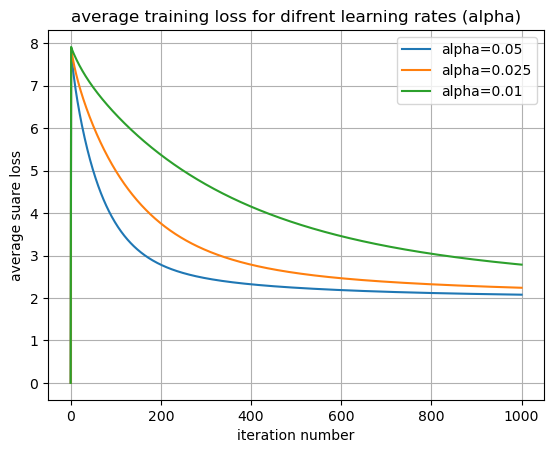
\includegraphics[width=10cm]{homework/homework_2/immages/12_1.png}
    \item 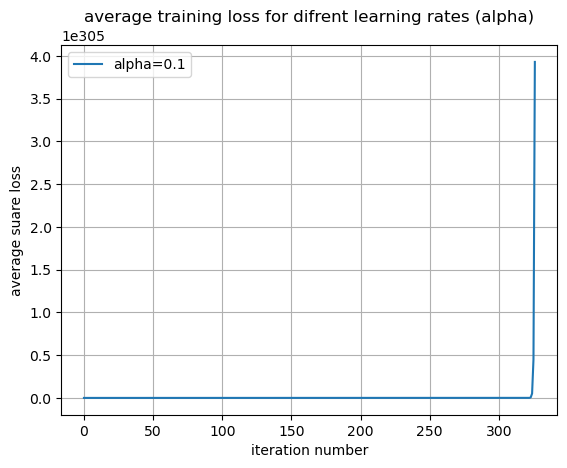
\includegraphics[width=10cm]{homework/homework_2/immages/12_2.png}
    
\end{itemize}

\item For the learning rate you selected above, plot the average test loss as a function of the iterations. You should observe overfitting: the test error first decreases and then increases.
\begin{itemize}

\item 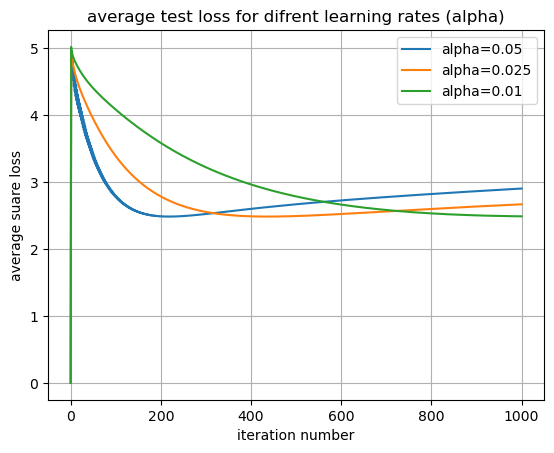
\includegraphics[width=10cm]{homework/homework_2/immages/13_1.png}
\item it seems the average learning rate in all values of$\alpha$ where we saw convergence law problem see decreases in test loss for a certain number of iterations and then increases after that which indicates over fitting 
\item 
\end{itemize}
\setcounter{saveenum}{\value{enumi}}
\end{enumerate}

\vspace{0.3cm}
\nyuparagrah{\bf Ridge Regression}

We will add $\ell_2$ regularization to linear regression. When we have a large number of features compared to instances, regularization
can help control overfitting. \emph{Ridge regression} is linear regression
with $\ell_{2}$ regularization. The regularization term is sometimes
called a penalty term. The objective function for ridge regression
is
\[
J_\lambda(\theta)=\frac{1}{m}\sum_{i=1}^{m}\left(h_{\theta}(\bs x_{i})-y_{i}\right)^{2}+\lambda\theta^{T}\theta,
\]
where $\lambda$ is the regularization parameter, which controls the
degree of regularization. Note that the bias term (which we included as an extra dimension in $\theta$) is being regularized
as well as the other parameters. Sometimes it is preferable to treat this term separately.

\begin{enumerate}
\setcounter{enumi}{\value{saveenum}}
\item Compute the gradient of $J_\lambda(\theta)$ and write down the expression
for updating $\theta$ in the gradient descent algorithm. (Matrix/vector
expression, without explicit summation)
\begin{itemize}
    \item $J_\lambda(\theta)=\frac{1}{m}\sum_{i=1}^{m}\left(h_{\theta}(\bs x_{i})-y_{i}\right)^{2}+\lambda\theta^{T}\theta=\frac{1}{m}||X\theta -y||_{2}^{2}+\lambda||\theta||_{2}^{2}$
    \item thus we can see that our gradient of ridge regression is $\nabla (J_{\lambda}(\theta))=\frac{2}{m}X^t(X\theta-y)+2\lambda\theta$
    \item thus our update rule becomes $\theta=\theta-\eta \nabla(J_{\lambda}(\theta))=\theta-\eta \nabla(\frac{2}{m}X^t(X\theta-y)+2\lambda\theta)$
\end{itemize}

\item Implement \texttt{compute\_regularized\_square\_loss\_gradient.}
\begin{itemize}
    \item \inputminted[firstline=182, lastline=198, breaklines=True]{python}{HW_2.PY.py}
\end{itemize}

    \item Implement \texttt{regularized\_grad\_descent.}
    \begin{itemize}
    \item \inputminted[firstline=203, lastline=228, breaklines=True]{python}{HW_2.PY.py}
\end{itemize}

\setcounter{saveenum}{\value{enumi}}
\end{enumerate}

Our goal is to find $\lambda$
that gives the minimum average square loss on the test set. So you should start your search very broadly, looking
over several orders of magnitude. For example, $\lambda\in\left\{ 10^{-7},10^{-5},10^{-3},10^{-1},1,10,100\right\} $.
Then you can zoom in on the best range. Follow the steps below to proceed.
\begin{enumerate}
\setcounter{enumi}{\value{saveenum}}
\item 
Choosing a reasonable step-size, plot training average square loss and
the test average square loss (just the average square loss part, without the regularization, in each case) as a function of the training iterations for various values of $\lambda$. What do you notice in terms of overfitting?
\begin{itemize}
\item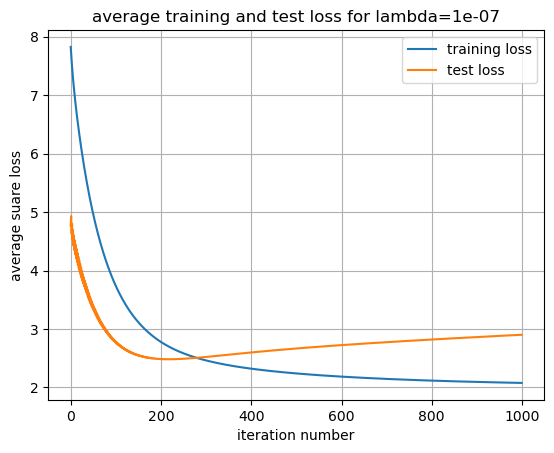
\includegraphics[width=10cm]{homework/homework_2/immages/17_1.png}
\item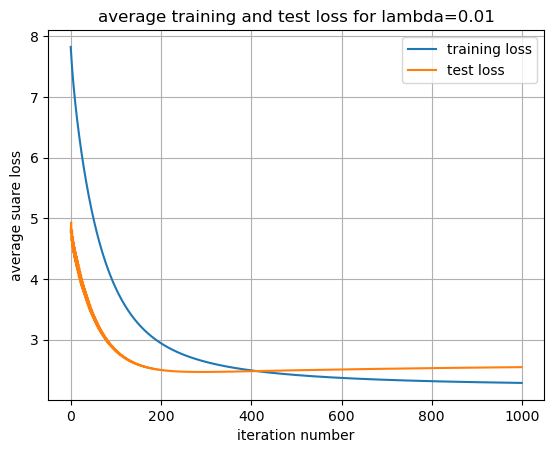
\includegraphics[width=10cm]{homework/homework_2/immages/17_2.png}
\item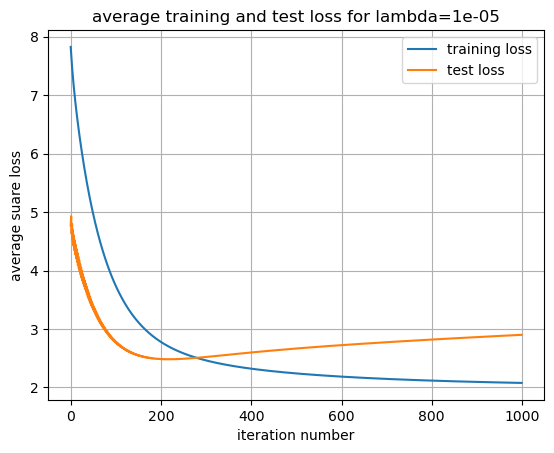
\includegraphics[width=10cm]{homework/homework_2/immages/17_3.png}
\item looking at these charts it seems like as  $\lambda$ grows the training and lest curve cross earlier meaning that our function is overfititng, more quickly with less training iterations 
\end{itemize}
\item Plot the training average square loss and
the test average square loss at the end of training as a function of $\lambda$. You may
want to have $\log(\lambda)$ on the $x$-axis rather than $\lambda$.
Which value of $\lambda$ would you choose ?  

\begin{itemize}
    \item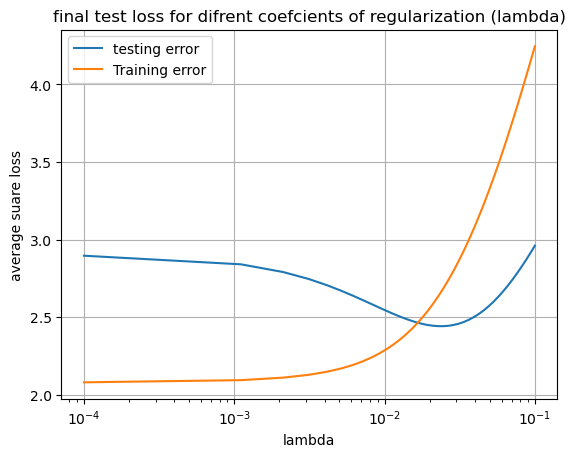
\includegraphics[width=10cm]{homework/homework_2/immages/18_1.png}
    \item this graph would seem to suggest a $\lambda$ around $10^{-2}$
\end{itemize}

\item Another heuristic of regularization is to \emph{early-stop} the training when the test error reaches a minimum. Add to the last plot the minimum of the test average square loss along training as a function of $\lambda$.
Is the value $\lambda$ you would select with early stopping the same as before? 
\begin{itemize}
    \item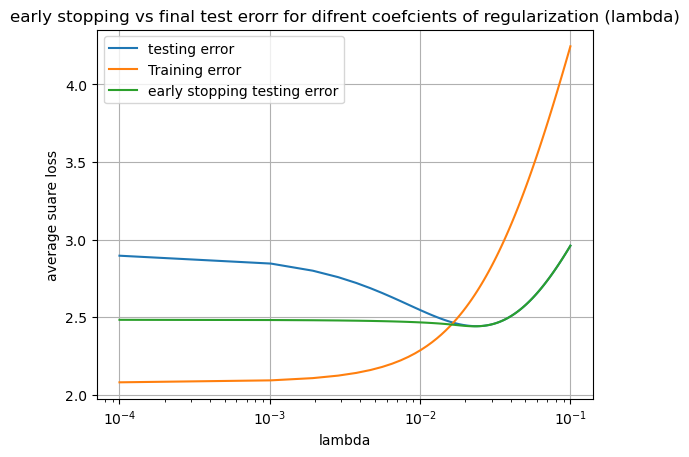
\includegraphics[width=10cm]{homework/homework_2/immages/19_1.png}
    \item they seem to suggest around the same amount. it is imporanat to note however that early stopping makes a very large differnnce for smaller values of $\lambda$
\end{itemize}

\item What $\theta$ would you select in practice and why?
\setcounter{saveenum}{\value{enumi}}
\begin{itemize}
    \item we have limited training data namely or $X_train$ is only 100 individuals, thus we need to be very care full about over fitting our training data. This makes regularization seem important 
    \item further we can see there are 49 features in our data set. This means we are trying to learn many features from little data, thus i would go with lasso regression, as it seems prudent in a case with so many features and such little data to try to learn the important features well, while avoiding over fitting to the training data. 
\end{itemize}


\end{enumerate}

\vspace{0.3cm}
\nyuparagrah{\bf Stochastic Gradient Descent (SGD) (optional)}

When the training data set is very large, evaluating the
gradient of the objective function can take a long time, since it
requires looking at each training example to take a single gradient
step. 

In SGD, rather than taking $-\nabla_{\theta} J(\theta)$
as our step direction to minimize 
\[
J(\theta)=\frac{1}{m}\sum_{i=1}^{m}f_{i}(\theta), 
\]
we take $-\nabla_\theta f_{i}(\theta)$ for some $i$
chosen uniformly at random from $\{1,\ldots,m\}$. The approximation
is poor, but we will show it is unbiased. 

In machine learning applications, each $f_{i}(\theta)$
would be the loss on the $i$th example. In
practical implementations for ML, the data points are randomly shuffled, and then we sweep through the whole training set one by
one, and perform an update for each training example individually.
One pass through the data is called an \emph{epoch}. Note that each
epoch of SGD touches as much data as a single step of batch gradient
descent. You can use the same ordering for each epoch, though optionally
you could investigate whether reshuffling after each epoch affects
the convergence speed. 
\begin{enumerate}
\setcounter{enumi}{\value{saveenum}}
\item Show that the objective function 
\[
J_{\lambda}(\theta)=\frac{1}{m}\sum_{i=1}^{m}\left(h_{\theta}(\bs x_{i})-y_{i}\right)^{2}+\lambda\theta^{T}\theta
\]
can be written in the form $J_\lambda(\theta)=\frac{1}{m}\sum_{i=1}^{m}f_{i}(\theta)$
by giving an expression for $f_{i}(\theta)$ that makes the two expressions
equivalent.

\begin{itemize}
    \item it is frailly obvious that using $f_i(\theta)=(h_{\theta}x_i-y_i)^2+\lambda\theta^{t}\theta$ we can maintain equality
\end{itemize}

\item Show that the stochastic gradient $\nabla_\theta f_{i}(\theta)$, for $i$
chosen uniformly at random from $\{1,\ldots,m\}$, is an \emph{unbiased estimator} of $\nabla_\theta J_\lambda(\theta)$. In other words, show that $\mathbb{E}\left[\nabla f_{i}(\theta)\right]=\nabla J_\lambda(\theta)$
for any $\theta$. It will be easier to prove
this for a general $J(\theta)=\frac{1}{m}\sum_{i=1}^{m}f_{i}(\theta)$,
rather than the specific case of ridge regression. You can start by
writing down an expression for $\mathbb{E}\left[\nabla f_{i}(\theta)\right]$
\begin{itemize}
    \item the expression $f_i(\theta)=(h_{\theta}x_i-y_i)^2+\lambda\theta^{t}\theta^{t}$ can be expanded as$f_i(\theta)=(h_{\theta}x_i-y_i)^2+\lambda\theta^{t}\theta= (h_{\theta}(x_i))^2-2h_{\theta}(x_i)+ y_i+y_i^2+\lambda\theta^{t}\theta^{t}$
    \item then taking the gradient of this expression we can see $\nabla f_i(\theta)=2 x_i^{T}x_i-2x_i^{t}y_i+2\lambda \theta$
    \item then we can take the expectation of this as  $E[\nabla f_i(\theta)]=E[2 x_i^{T}x_i-2x_i^{t}y_i+2\lambda \theta]$ everything is constant except for $x_i,y_i$ thus $E[\nabla f_i(\theta)]=2\thetaE[ x_i^{t}x_i]-2E[x_i^{t} y_i]+2\lambda \theta] $
    \item then we can see that $2\theta E[ x_i^{t}x^{i}]=2\Sigma_{i=1}^{n}x_i^{t}x_iP(x_i=i)$ and as $P(x_i=i)$ uniformly distributed we can write$2\theta E[ x_i^{t}x_i]=2\Sigma_{i=1}^{n}x_i^{t}x_iP(x_i=i)=\frac{1}{n}\Sigma_{i=1}^{m}x_i^{t}x_i$
    \item similar logic tells us that $[x_i^{t}y_i]=\frac{1}{m}\Sigma_{i=1}^{m}x_i^{t}y_i$
    \item so thus  $E[\nabla f_i(\theta)]=2\theta E[ x_i^{t}x_i]-2E[x_i^{t} y_i]+2\lambda \theta]=2(\theta \frac{1}{n}\Sigma_{i=1}^{m}x_i^{t}x_i-\frac{1}{m}\Sigma_{i=1}^{m}x_i^{t}y_i+\lambda h_{\theta})=2\frac{1}{n}\Sigma_{i=1}^{m} x_i^{t}x_i-x_i^{t}y_i)+2\lambda \theta$
    \item we can also see that $\nabla(J_{\lambda}(\theta))=\frac{1}{m}\Sigma_{i=1}^{m}2(x_i)^{t}x_i-2x_i^{t}y_i+2\lambda \theta$
    \item thus we see $E[\nabla f_i(\theta)]=\nabla(J_{\lambda}(\theta))$ which was what we wanted to show
\end{itemize}

\item Write down the update rule for $\theta$ in SGD for the ridge
regression objective function.
\begin{itemize}
    \item we can write stochastic gradient descent in general as $\theta\leftarrow \theta - \alpha \nabla_{\theta}\ell(h_{\theta}x_i,y_i))$
    \item so in the case of ridge regression it is   $\theta\leftarrow \theta - \alpha(2\frac{1}{n}h_{\theta} x_i^{t}x_i-x_i^{t}y_i)+2\lambda \theta)$
\end{itemize}

\item Implement \texttt{stochastic\_grad\_descent}. 
\begin{itemize}
    \item \inputminted[firstline=235, lastline=274, breaklines=True]{python}{HW_2.PY.py}
\end{itemize}



\item Use SGD to find $\theta_{\lambda}^{*}$ that minimizes the ridge regression
objective for the $\lambda$ you selected in the previous
problem. (If you could not solve the previous problem, choose $\lambda=10^{-2}$). Try a few fixed step sizes (at least try $\eta_{t}\in\left\{ 0.05,.005\right\} $).
Note that SGD may not converge with fixed step size. Simply note your
results. Next try step sizes that decrease with the step number according
to the following schedules: $\eta_{t}=\frac{C}{t}$ and $\eta_{t}=\frac{C}{\sqrt{t}}$, $C \leq 1$. Please include $C = 0.1$ in your submissions. You are encouraged to try different values of $C$ (see notes below for details).
For each step size rule, plot the value of the objective function
(or the log of the objective function if that is more clear) as a
function of epoch (or step number, if you prefer). How do the results compare?
\begin{itemize}
    \item it does not seem like fixed $\alpha$ values are able to converge very well for me.
    \item 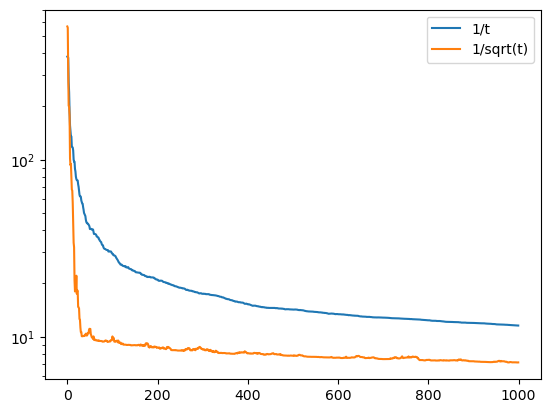
\includegraphics[width=10cm]{homework/homework_2/immages/25_1.png}
    \item it seems that using $\alpha=\frac{c}{t}$ the values of $\theta$ reaches a point where it converges very quickly but that point does not necessarily get training error as low as it can go
    \item it seems that using $\alpha=\frac{c}{\sqrt{t}}$ the values of $\theta$ reach near convergence a bit more slowly, but result in a lower training loss in the long term
    
\end{itemize}
\setcounter{saveenum}{\value{enumi}}
\end{enumerate}

A few remarks about the question above:
\begin{itemize}
\item In this case we are investigating the convergence rate of
the optimization algorithm with different step size schedules, thus
we're interested in the value of the objective function, which includes
the regularization term.
\item Sometimes the initial step size ($C$
for $C/t$ and $C/\sqrt{t}$) is too aggressive and will get you into
a part of parameter space from which you can't recover. Try reducing $C$ to counter this problem. 
\item SGD
convergence is much slower than GD once we get close to the minimizer
(remember, the SGD step directions are very noisy versions of the
GD step direction). If you look at the objective function values on
a logarithmic scale, it may look like SGD will never find objective
values that are as low as GD gets. In statistical learning theory terminology, GD has much smaller \emph{optimization} error than SGD. However,
this difference in optimization error is usually dominated by other
sources of error (estimation error and approximation error). Moreover,
for very large datasets, SGD (or minibatch GD) is much faster (by
wall-clock time) than GD to reach a point close enough
to the minimizer. 
\end{itemize}

{\bf Acknowledgement:} This problem set is based on assignments developed by David Rosenberg of NYU and Bloomberg.


\section{\large Image classification with regularized logistic regression}


{\color{nyupurple} \large \bf Dataset}  

In this problem set we will examine a classification problem. To do so we will use the MNIST dataset\footnote{\url{http://yann.lecun.com/exdb/mnist/}} which is one of the traditional image benchmark for machine learning algorithms. We will only load the data from the 0 and 1 class, and try to predict the class from the image. You will find the support code for this problem in \texttt{mnist\_classification\_source\_code.py}.
Before starting, take a little time to inspect the data. Load \texttt{X\_train, y\_train, X\_test, y\_test} with \texttt{pre\_process\_mnist\_01()}. Using the function \texttt{plt.imshow} from \texttt{matplotlib} visualize some data points from \texttt{X\_train} by reshaping the $784$ dimensional vectors into $28 \times 28$ arrays. Note how the class labels `0' and `1' have been encoded in \texttt{y\_train}. No need to report these steps in your submission.


{\color{nyupurple} \large \bf Logistic regression}  

We will use here again a linear model, meaning that we will fit an affine function,
\[
h_{\theta, b}(\bs x) = \theta^T\bs x + b,
\]
with $\bs x \in \mathbb{R}^{784}$, $\bs \theta \in \mathbb{R}^{784}$ and $b\in \mathbb{R}$.
This time we will use the logistic loss instead of the squared loss. Instead of coding everything from scratch, we will also use the package \texttt{scikit learn} and study the effects of $\ell_1$ regularization. You may want to check that you have a version of the package up to date (0.24.1).

\begin{enumerate}
\setcounter{enumi}{\value{saveenum}}
  \item Recall the definition of the logistic loss between target $y$ and a prediction $h_{\theta, b}(\bs x)$ as a function of the margin $m = y h_{\theta, b}(\bs x)$. Show that given that we chose the convention $y_i\in\{-1,1\}$, our objective function over the training data $\{\bs x_i, y_i\}_{i=1}^m$ can be re-written as
  \[
    L(\theta) = \frac 1 {2 m} \sum_{i=1}^m  (1 + y_i) \log ( 1 + e^{- h_{\theta, b}(\bs x_i)}) +  (1 - y_i) \log(1 + e^{h_{\theta, b}(\bs x_i)}).
    \]
\begin{itemize}
    \item recall that logistic loss can be written as $\ell_{log}=log(1+e^{-(y h_{\theta, b}(\bs x))})$
    \item we can think of the risk over our dataset $\{\bs x_i, y_i\}_{i=1}^m$ as $\frac{1}{m}\Sigma_{i=1}^{m}\ell(x_i,y_i)$ given we are using logistic loss this becomes $\frac{1}{m}\Sigma_{i=1}^{m} log(1+e^{-(y_i h_{\theta, b}(\bs x_i))})$
    \item further note that for any given data point $\frac 1 {2}\ell_{log}(x_i,y_i)=(1 + y_i) \log ( 1 + e^{- h_{\theta, b}(\bs x_i)}) +  (1 - y_i) \log(1 + e^{h_{\theta, b}(\bs x_i)})$ given $y_i,h_{\theta, b}(\bs x_i) \in \{-1,1\} $ to show we can check all values that this expression can take
    \begin{itemize}
        \item suppose $y_i=1,h_{\theta, b}(\bs x_i)=1$ then $(1 + y_i) \log ( 1 + e^{- h_{\theta, b}(\bs x_i)}) +  (1 - y_i) \log(1 + e^{h_{\theta, b}(\bs x_i)})=(2) \log ( 1 + e^{-1}) +  (0) \log(1 + e^{1})=(2) \log ( 1 + e^{-1})$ while   $\frac{1}{2}log(1+e^{-(y_i h_{\theta, b}(\bs x_i))})=\frac{1}{2}log(1+e^{-1})$
        \item suppose $y_i=1,h_{\theta, b}(\bs x_i)=-1$ then $(1 + y_i) \log ( 1 + e^{- h_{\theta, b}(\bs x_i)}) +  (1 - y_i) \log(1 + e^{h_{\theta, b}(\bs x_i)})=(2) \log ( 1 + e^{1}) +  (0) \log(1 + e^{-1})=(2) \log ( 1 + e^{1})$ while   $\frac{1}{2}log(1+e^{-(y_i h_{\theta, b}(\bs x_i))})=\frac{1}{2}log(1+e^{1})$
                \item suppose $y_i=-1,h_{\theta, b}(\bs x_i)=-1$ then $(1 + y_i) \log ( 1 + e^{- h_{\theta, b}(\bs x_i)}) +  (1 - y_i) \log(1 + e^{h_{\theta, b}(\bs x_i)})=(0) \log ( 1 + e^{1}) +  (2) \log(1 + e^{-1})=(2) \log ( 1 + e^{-1})$ while   $\frac{1}{2}log(1+e^{-(y_i h_{\theta, b}(\bs x_i))})=\frac{1}{2}log(1+e^{-1})$
    \item finally suppose $y_i=-1,h_{\theta, b}(\bs x_i)=1$ then $(1 + y_i) \log ( 1 + e^{- h_{\theta, b}(\bs x_i)}) +  (1 - y_i) \log(1 + e^{h_{\theta, b}(\bs x_i)})=(0) \log ( 1 + e^{1}) +  (2) \log(1 + e^{1})=(2) \log ( 1 + e^{1})$ while   $\frac{1}{2}log(1+e^{-(y_i h_{\theta, b}(\bs x_i))})=\frac{1}{2}log(1+e^{1})$
    \end{itemize}
\item thus we can see that $\frac{1}{2m}(\Sigma_{i=1}^{M}(1 + y_i) \log ( 1 + e^{- h_{\theta, b}(\bs x_i)}) +  (1 - y_i) \log(1 + e^{h_{\theta, b}(\bs x_i)})=(0) \log ( 1 + e^{1}) +  (2) \log(1 + e^{1})$ which was the realtion we wanted to show
\end{itemize}


  \item What will become the loss function if we regularize the coefficients of $\theta$ with an $\ell_1$ penalty using a regularization parameter $\alpha$ ?

  \begin{itemize}
      \item adding an $\ell_{1}$ pelaty with parameter $\alpha$ our loss function becomes     $L(\theta) = \frac 1 {2 m} \sum_{i=1}^m  (1 + y_i) \log ( 1 + e^{- h_{\theta, b}(\bs x_i)}) +  (1 - y_i) \log(1 + e^{h_{\theta, b}(\bs x_i)})+\alpha|\theta|_{1}.$
  \end{itemize}
  

\setcounter{saveenum}{\value{enumi}}
\end{enumerate}

We are going to use the module \texttt{SGDClassifier} from scikit learn. In the code provided we have set a little example of its usage. By checking the online documentation\footnote{\url{https://scikit-learn.org/stable/modules/generated/sklearn.linear_model.SGDClassifier.html}}, make sure you understand the meaning of all the keyword arguments that were specified. We will keep the learning rate schedule and the maximum number of iterations fixed to the given values for all the problem. Note that scikit learn is actually implementing a fancy version of SGD to deal with the $\ell_1$ penalty which is not differentiable everywhere, but we will not enter these details here.

\begin{enumerate}
\setcounter{enumi}{\value{saveenum}}
  \item To evaluate the quality of our model we will use the classification error, which corresponds to the fraction of incorrectly labeled examples. For a given sample, the classification error is 1 if no example was labeled correctly and 0 if all examples were perfectly labeled. 
  Using the method \texttt{clf.predict()} from the classifier write a function that takes as input an \texttt{SGDClassifier} which we will call \texttt{clf}, a design matrix \texttt{X} and a target vector \texttt{y} and returns the classification error. You should check that    your function returns the same value as \newline \texttt{1 - clf.score(X, y)}.
\begin{itemize}
    \item \inputminted[firstline=235, lastline=274, breaklines=True]{python}{HW_2.PY.py}
\end{itemize}
  
\setcounter{saveenum}{\value{enumi}}
\end{enumerate}


To speed up computations we will subsample the data. Using the function \texttt{sub\_sample}, restrict \texttt{X\_train} and \texttt{y\_train} to \texttt{N\_train = 100}. 

\begin{enumerate}
\setcounter{enumi}{\value{saveenum}}
  \item Report the test classification error achieved by the logistic regression as a function of the regularization parameters $\alpha$ (taking 10 values between $10^{-4}$ and $10^{-1}$). You should make a plot with $\alpha$ as the x-axis in log scale. For each value of $\alpha$, you should repeat the experiment 10 times so has to finally report the mean value and the standard deviation. You should use \texttt{plt.errorbar} to plot the standard deviation as error bars.

  \begin{itemize}
      \item 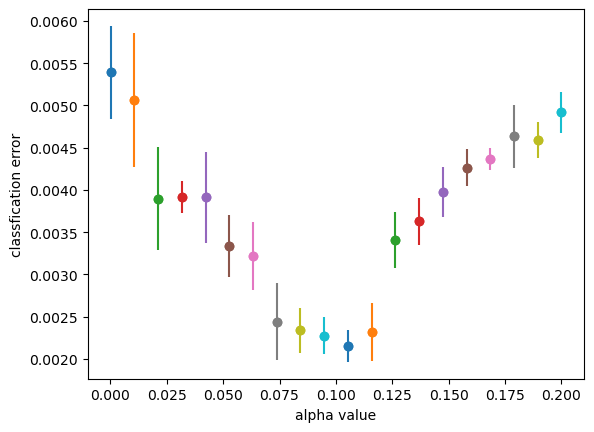
\includegraphics[width=10cm]{homework/homework_2/immages/29_1.png}
      \item i chose to widen the the search range of alpha a bit, since i think it makes the overall trend more clear
      \item namely that reducing $\alpha$ only causes lower average and standard deviation in classification error to a point, after which these metric increase again
  \end{itemize}
  
  \item Which source(s) of randomness are we averaging over by repeating the experiment?
\begin{itemize}
    \item our estimator is based on stochastic gradient descent, repeating the experiment 10 times, at each alpha level helps reduce sampling uncertainty and thus approximation error
\end{itemize}
  
  \item What is the optimal value of the parameter $\alpha$ among the values you tested? 

  \begin{itemize}
      \item it looks like .01 is the optimal value of  $\alpha$
  \end{itemize}

  \item Finally, for one run of the fit for each value of $\alpha$ plot the value of the fitted $\theta$. You can access it via \texttt{clf.coef\_}, and should reshape the $784$ dimensional vector to a $28\times 28$ arrray to visualize it with \texttt{plt.imshow}. Defining \texttt{scale = np.abs(clf.coef\_).max()}, you can use the following keyword arguments (\texttt{cmap=plt.cm.RdBu, vmax=scale, vmin=-scale}) which will set the colors nicely in the plot. You should also use a \texttt{plt.colorbar()} to visualize the values associated with the colors.
  
  \item What can you note about the pattern in $\theta$? What can you note about the effect of the regularization?

  \begin{itemize}
    \item 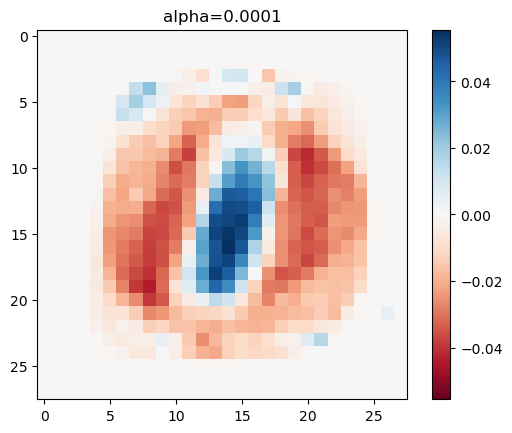
\includegraphics[width=10cm]{homework/homework_2/immages/32_1.png}
    \item 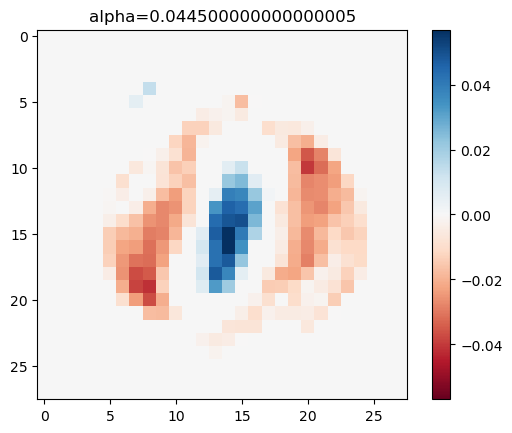
\includegraphics[width=10cm]{homework/homework_2/immages/32_2.png}
    \item 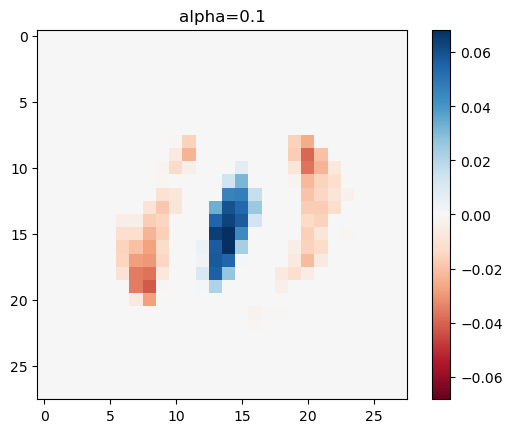
\includegraphics[width=10cm]{homework/homework_2/immages/32_3.png}
    \item as can be seen from this subset of the images over the range 
       higher values of $\alpha$ tend to have less color implying that more of the coefficients are close to zero which makes sense because we are using $\ell_{1}$ regularization with a stronger regularization term and thus will get a sparse estimator
  \end{itemize}

  
\setcounter{saveenum}{\value{enumi}}
\end{enumerate}

\end{document}
